% Generated by Sphinx.

\documentclass[a4paper,11pt,english]{article}
\usepackage[utf8]{inputenc}
\usepackage[T1]{fontenc}
\usepackage{xfrac}
%\usepackage[none]{hyphenat}
\usepackage{babel}
\usepackage{times}
\usepackage[Bjarne]{fncychap}
\usepackage{multirow}
\usepackage[hidelinks,colorlinks=true,urlcolor=blue,linkcolor=black,]{hyperref}
\usepackage[all]{hypcap}
\usepackage{graphicx}
\usepackage{float}
\newcommand{\reg}{\textsuperscript{\textregistered}} 
\usepackage{subcaption}

\title{ASSIsT: An Automatic SNP ScorIng Tool for in and out-breeding species\\
Reference Manual}
\date{\textbf{Version 1.02}\\ \today}
%\release{1.0}
\author{Di Guardo M,
Micheletti D,
Bianco L,
Koehorst-van Putten HJJ,\\
Longhi S,
Costa F,
Aranzana MJ,
Velasco R,
Arús P,\\
Troggio M,
van de Weg WE
}

\begin{document}

\maketitle
\tableofcontents
%\phantomsection\label{index::doc}

\newpage
\textbf{ASSIsT} is a tool for efficient filtering of Illumina Infinium/BeadExpress based SNP
markers. This software can analyse different types of experimental populations: Cross-pollinated
(CP – F1), Back Cross (BC), F2 and collections of unrelated individuals (Germplasm). It is possible
to export the filtered data in several formats according to the most widely used software for
marker-trait association analysis.



\section{Getting started}
\label{index:getting-started}\label{
index:assist-an-automatic-snp-scoring-tool-for-in-and-out-breeding-species}
ASSIsT is written in Python; therefore, it can run virtually in any platform with python installed.


\subsection{Availability}
\label{index:availability}
Source code and  Windows executables (built using pyinstaller) are available for download at:
\begin{itemize}
 \item \href{http://compbiotoolbox.fmach.it/assist}{http://compbiotoolbox.fmach.it/assist} 
 \item \href{http://bioinformatics.tecnoparco.org/fruitbreedomics/assist-tool}{
http://bioinformatics.tecnoparco.org/fruitbreedomics/assist-tool}
\end{itemize}



When using ASSIsT, please cite:
Di Guardo and Micheletti et al. 2015, 
referenced as:
Di Guardo M, Micheletti D, Bianco L, Koehorst-van Putten HJJ, Longhi S, Costa F, Aranzana MJ,
Velasco R, Arús P, Troggio M, van de Weg EW (XXXX) ASSIsT: An Automatic SNP ScorIng Tool for in- and
out-breeding species. Bioinformatics, DOI: 10.1093/bioinformatics/btv446

\subsection{What's new in version 1.02}
\label{index:{What's new in version 1.02}}
\begin{itemize}
\item Fixed the shift of two individuals in the gtypes.csv output file with Germplasm population type.
\end{itemize}




\subsection{Installing ASSIsT}
\label{index:installing-assist}
The Windows executables is distributed as a zip archive. It not necessary to install ASSIsT, just
extract the ASSIsT\_Windows.xx.zip archive (xx is the version number).

The source code is a collection of Python scripts. They can be executed from any operating system
with
Python 2.7 installed. The following additional Python modules are needed to run the software:
\begin{itemize}
\item PyQt4 (v.4.8 or higher)
\item NumPy (v.1.8 or higher)
\item matplotlib (v.1.3 or higher)
\item SciPy (v.0.14 or higher)
\end{itemize}


\subsection{Running ASSIsT}
\label{index:running-assist}
In Windows, double click on {\ttfamily{ASSIsT.exe}} to start ASSIsT.
To run ASSIsT from the source code execute {\ttfamily{ASSIsT.py}} from a command line shell.
\begin{figure}[H]
\centering
\capstart

\scalebox{0.500000}{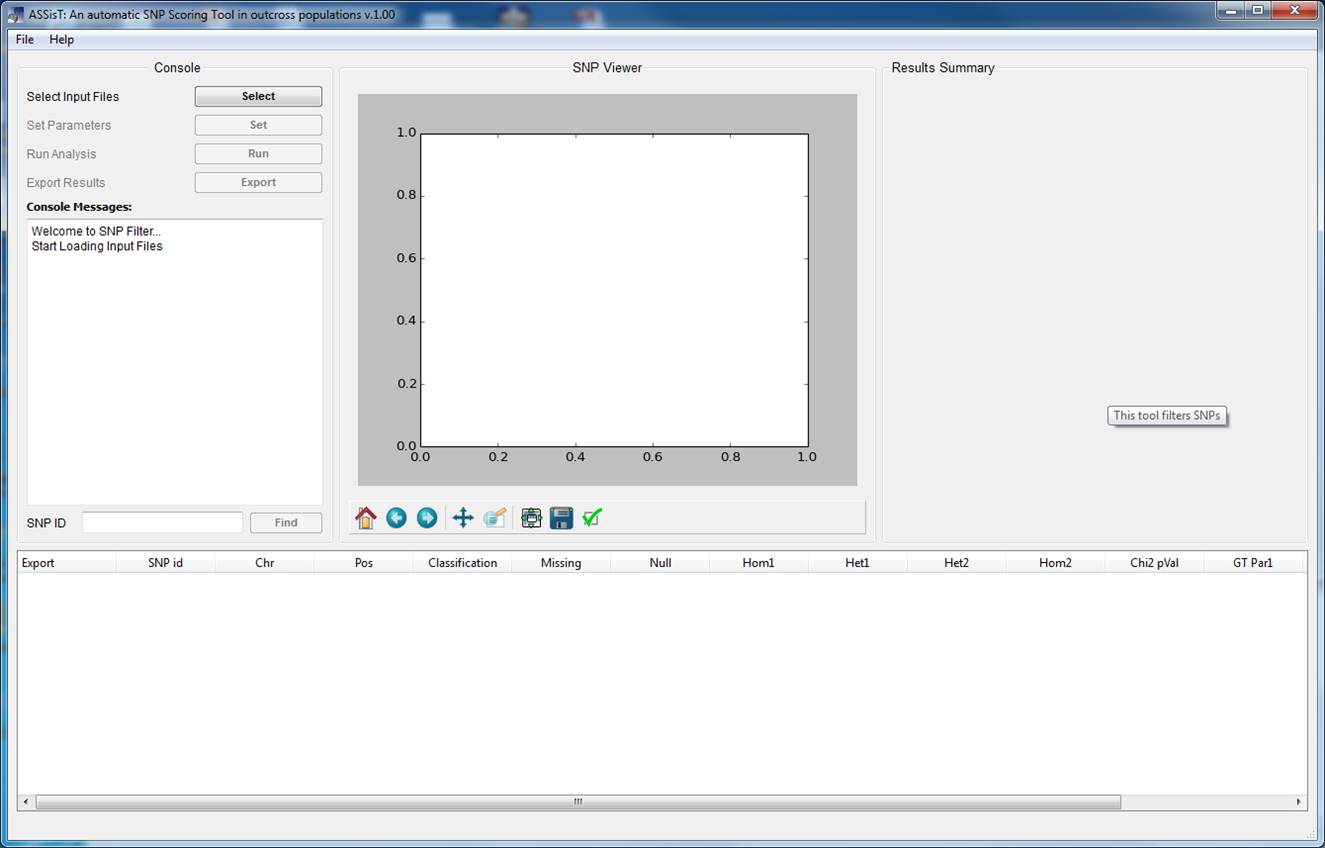
\includegraphics{_picture/mainwin.jpg}}
\caption{ASSIsT layout.}\end{figure}

The analysis start by loading the four input files (GenomeStudio\reg~Final Report,
Genome Studio\reg~DNA Report, pedigree, and map file) using the \textbf{Select} button. Example data
files are available at the previously mentioned web-pages. Example data are provided for Cross
Pollinators (CP) and  F2-germplasm (F2 for inbreeding crops). Please note
that the map file is not mandatory. To load the files
click on \scalebox{0.600000}{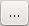
\includegraphics{_picture/loadfile.png}} and select the appropriate input file 
or enter the file name (with the full path)
in the text box.
\begin{figure}[H]
\centering
\capstart

\scalebox{0.500000}{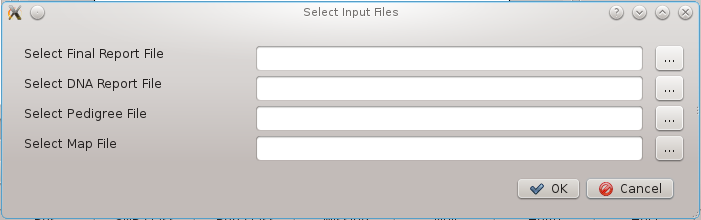
\includegraphics{_picture/loadfile_win.png}}
\caption{Menu opened by clicking on the Select button}\end{figure}

After the Input files are correctly imported, it is necessary to set up the filtering parameters
by clicking on the \textbf{Set} button. The first parameter to set is the population type
(``CP (F1)'', BC, F2 or Germplasm) and then the related statistical and germplasm parameters
(see below for details).
\begin{figure}[H]
\centering
\capstart

\scalebox{0.600000}{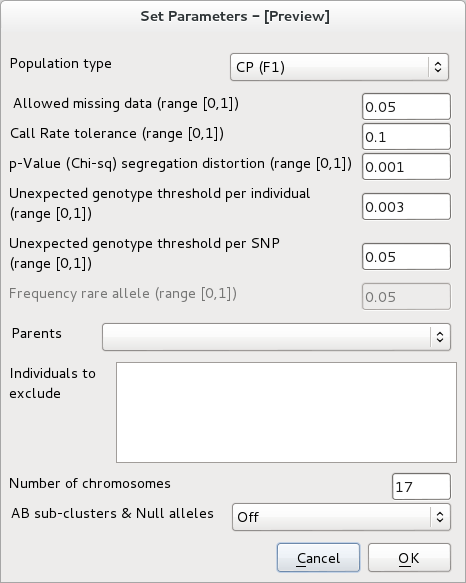
\includegraphics{_picture/setparam_annotated.png}}
\caption{Dialog to select analysis parameter.}\end{figure}

When this step is completed, the \textbf{Run} button becomes available, and the analysis can be
performed by clicking on it.

At the end of the analysis, it is possible to choose the files to export by clicking \textbf{Export}
Some outputs provide more detailed information on the performance of the filtering analysis itself,
e.g.,
``Summary'', ``Custom gtypes'', ``Custom SNP information table'' and ``Custom Mendel error report''.
\begin{figure}[H]
\centering
\capstart

\scalebox{0.500000}{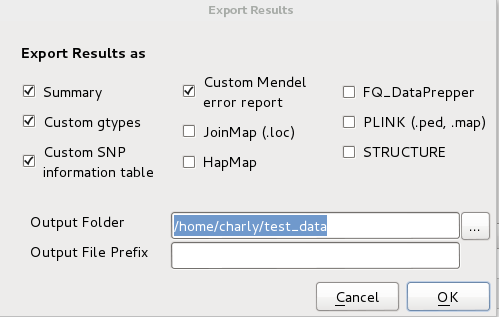
\includegraphics{_picture/export_win.png}}
\caption{Dialog to select the files to Export.}\end{figure}

Additionally, it is possible to export the results in additional formats (JoinMap\reg, PLINK,
HapMap, FlexQTL\texttrademark  DataPrepper and STRUCTURE) that can be used as inputs to third-party
programmes.

Note: Through the export section,  a customized prefix can be added to the names of the
output files.


\section{Input files}
\label{index:input-files}
Sample and marker names have to be consistent in all 4 input files.
\begin{description}
 \item [Genome Studio Final Report:]
Using the Report Wizard (Open \textbf{GenomeStudio\reg}\\ $\rightarrow$ \textbf{Analysis}
$\rightarrow$ \textbf{Reports} $\rightarrow$ \textbf{Report wizard}), select \textbf{Final
Report}, and press \textbf{Next}. On the following page, use the \textbf{``redo with the best 10th
Percentile GC Score''}
option, and
press \textbf{Next}. If some samples have been excluded from the GenomeStudio\reg~ project you
need
to remove
or zero-out your sample in the report. Make your choice according to how you want to account 
the excluded data and press \textbf{Next} (if no samples have been excluded from GenomeStudio\reg~
project this page is not displayed).
The format of the Final  Report must be set to ``Standard'' (the other choices are ``Matrix''
or ``3rd Party''). The Final Report should include the following columns (in the specified order):
\begin{enumerate}
\item SNP Name
\item Sample ID
\item Allele1 - Top (or Allele1-AB or Allele1-design, depending on the desired type of output)
\item Allele2 - Top (or Allele2-AB or Allele2-design, has to be in line with the choice for
Allele1)
\item GC Score
\item GT Score
\item Theta
\item R
\end{enumerate}

Select \textbf{Group by SNP} (and not by ``sample''). In \textbf{General Option}, select ``Tab'' as
the field delimiter.
Press \textbf{Next}, and select the folder in which the file has to be stored, and enter its name.
Press \textbf{Finish}.

\item [DNA Report:]
Using the Genome Studio Report Wizard (see the above section on the GenomeStudio\reg~  Final Report)
select  \textbf{DNA Report}. Press  \textbf{Next} once or twice (twice if there are excluded samples
in the GenomeStudio\reg~  project). Use the \textbf{redo with the best 10th Percentile GC Score}
option and press  \textbf{Next} once or twice. Finally select \textbf{SampleID}.

\item [Pedigree:]
The pedigree file is composed of 3 columns: The first contains the list of individuals to analyse,
while in the second and third columns, the female and male parents are reported.
Be aware that this order (sample, mother, father) is important for some of the output files and
that the only compulsory column is the first. 
Tabulation (``tab'') must be used as the field
delimiter. The file must also include the following header row:
\begin{quote}

//SampleID Mother Father
\end{quote}

Sample names should not include white spaces (blanks) or special characters (non-ASCII symbols,
\href{http://it.wikipedia.org/wiki/ASCII}{http://it.wikipedia.org/wiki/ASCII}).

\item[Map file (Optional):]
The map file specifies the physical or genetic  coordinates of the Genotyped SNPs. This file has to include three columns:
the SNPid, the chromosome, and the position. The position can be expressed in base pairs (bp),
Megabase (Mb), or centiMorgan (cM).
The following file header line is necessary:
\begin{quote}

//SNPid Chromosome Position
\end{quote}
\end{description}

\section{Customizable parameters}
\label{index:customizable-parameters}
\begin{description}
 \item [Population type:] Type of population analysed. The possible choices are ``CP
(F1)'', ``BC'', ``F2''
and ``Germplasm''. The Back-cross (BC) population is analysed as Cross-pollinated (CP) population,
as the segregation types are the same (ABxAA or ABxAB and occasionally ABxAC=EFxEG). This tool does
not make any assumption on the Grand-parental origin of the alleles.

\item [Allowed missing data:] Frequency of allowed missing data (No Call) by SNP and by
individuals.
The default value is 0.05. Range {[}0,1{]}.

\item [Call Rate tolerance:]  Maximum tolerance for the  distance between an individual
call rate and
the analysed population mean. This parameter is used to exclude individuals (rather than SNP
markers)
for which too many SNPs could not be called. The default value is 0.1. Range {[}0,1{]}

\item [p-Value (Chi-sq) segregation distortion:] p-value of the Chi-squared test to test
the allelic segregation. This check is based on the Hardy-Weinberg equilibrium test for
unstructured germplasm or the expected and observed segregation ratio's when bi-parental
populations are
analysed. The lower the threshold, the more distortion is allowed.
The default value is 0.001. Range {[}0,1{]}.

\item [Unexpected genotype threshold per individual:] Proportion of allowed unexpect-ed genotypes
for each individual (Trio's Mendel Errors). This parameter is applied at a very
final stage of the filtering process, after having accounted for "AB-
sub-clusters and Null alleles" (see below) and is used to exclude 
individuals that have high probability to be not true to type or that 
have erroneous pedigree records.
The default value is 0.003. Range {[}0,1{]}.

\item [Unexpected genotype threshold per SNP:] Proportion of allowed unexpected \\genotypes for each
SNP (Trio's Mendel Errors). Unexpeced calls will be made missing as long as their proportion does
not exceed this threshold. When the threshold is exceeded, this SNP will be excluded. Note that this
option is only available when Population Type ``CP
(F1)'', ``BC'' or ``F2'' is selected. The default value is 0.05. Range {[}0,1{]}.

\item [Frequency rare allele:] Maximum frequency to define an allele as rare. Note that this option
is only available when Population Type ``Germplasm'' is selected. The default value is 0.05. Range
{[}0,1{]}.

\item [Parents:] Parents (``CP (F1)'', BCx) or grandparents (F2) of the analysed
experimental population.
This parameter is used to specify which segregating family will be analysed.
Note that this option is not available when germplasm is selected as Population type.

\item [Individuals to exclude:] It is possible to select the individuals to remove prior
to the
filtering analysis.

\item [Number of chromosomes:] Chromosome number of the species in the analysis. Since the
tool was developed for apple, the default value is 17.

\item [AB sub-clusters \& Null alleles:] Find and score markers with the AB cluster
split into two sub-clusters and
markers that show a null-allele.
Note that this option is only available when Population Type ``CP (F1)'' or ``BC'' is selected.
\end{description}

\section{Output files format}
\label{index:output-files-format}
\begin{description}
 \item [summary.txt:] Gives an overview of the assay performances both
by markers (number of markers for each class) and by individuals
(number of samples analysed and list of individuals that did not pass
the quality check: outcross or individuals with poor DNA quality).  Moreover,
it presents the data and parameter settings that were used for the analyses.

\item [gtypes.csv:] Custom file reporting the genotypes of all the successfully genotyped
SNPs
for each individual in the pedigree file. Each row represents an SNP. The individuals of
the analysed population are sorted lexicographically, and the identified outcrosses are reported at
the end of each row. The file contains the following information:
SNP name (SNP id), Chromosome (Chr) position (Pos), Classification of SNP performance (Classification),
Number of No Calls (Missing), number of individuals for each genotype (HomozygousNull, Hom1,
Het1, Het2, Hom2), Chi-Squared p-value and the genotypes for each individual analysed.
Note that Hom stands for homozygous (\emph{AA} or \emph{BB}), Het for heterozygous (\emph{AB}, \emph{Ab}, \emph{aB}, \emph{AO}, \emph{BO})
and HomozygousNull for the contemporary presence of a null allele in both
chromosomes (\emph{OO}). \emph{O} is used to indicate a null allele while a lowercase \emph{a} or
\emph{b} indicates the presence of an additional SNP at the \emph{A} or \emph{B} probe site,
respectively.

\item [mendel\_error.tsv:] For each unexpected genotype, the individual involved is
specified together
with the genotypes of the two parents and the marker name (only for ``CP (F1)'', BCx or F2, and for
the SNP that passed filtering).

\item [snp\_table.csv:] Reports the segregation and classification information for each
SNP
(excluded and included). Each line reports the information for a single SNP in the following order:
SNP id, genetic position (Chr and Pos), whether the marker has been exported (Exported),
Classification of SNP performance (Classification), number of missing values (Missing), number of
individuals
for each allelic class (HomNull, Hom1, Het1, Het2, Hom2), Chi-Squared p-value. The genotype of the
parents (GT Par1,GT Par2) is reported  only when an experimental population is analysed, while
the MAF information is provided only when a
Germplasm set is analysed. Het2 represents the second heterozygous
state and is present only for the SNPs with \emph{AB} cluster showing a significant split in two
sub-clusters or for the \emph{A0 x BO}  cross.

\item [joinmap.loc:]  Input file for JoinMap\reg~. This file is created
only for the CP population. More details on the file format are available on the
\href{http://www.kyazma.nl/docs/JM4manual.pdf}{JoinMap\reg~} user manual beginning on 
page 46. This file contains only the ``approved'' markers while the ``discarded'' markers are
left out.

\item [flexQTL DataPrepper:] This output is helpful when preparing an input file for
FlexQTL\texttrademark.

\item [PLINK:] Creates the ped and map file that can be used as an input for PLINK
(\href{http://pngu.mgh.harvard.edu/~purcell/plink}{Purcell} et al. 2007);
this file includes all the SNPs that pass the quality filtering. Details on the file format can be
found at
\href{http://pngu.mgh.harvard.edu/~purcell/plink/data.shtml}{
pngu.mgh.harvard.edu/~purcell/plink/data.shtml}.

\item [HapMap:] creates a file including all the SNPs that pass the quality filtering.
File format specifications can be found at 
\href{
https://www.broadinstitute.org/science/programs/medical-and-population-genetics/haploview/input-file
-formats-0}{www.broadinstitute.org}.

\item [Structure:] Input file for
\href{http://pritchardlab.stanford.edu/structure.html}{Structure}. The file includes two header
lines with the marker
position and the relative distance between them. Each individual is stored in a single line. The
missing data are coded as `-9', while the nucleotides are stored as digits (\emph{1=A, 2=C, 3=G,
4=T}).
\end{description}


\section{SNP classification}
\label{index:snp-classification}\label{index:structure}
A pre-screening of the fully genotyped germplasm is performed  to identify poorly performing
SNPs and individuals with low DNA quality. In this first phase all the SNPs showing more than 75\%
of NoCall in GenomeStudio\reg~  are classified as Failed and excluded from further analysis.
Additionally,
the accessions showing a CallRate lower than the average CallRate minus the ``Call Rate tolerance''
are also excluded.
The remaining SNPs are further classified based on their performances on the accessions from
the pedigree file.

\begin{description}
 \item [Robust:] All the successfully genotyped SNPs in which the segregation follows
Mendelian rules and the number of NoCall is lower
than the maximum allowed in the dataset. In ``CP (F1)'' and ``BC'' populations, the SNPs can be 
segregated into two or three clusters depending on the parent genotype (\emph{AA*x*AB} and
\emph{AB*x*AB}). In ``F2'' and ``Germplasm'', populations, the SNPs
show three clusters with a not significant p-value for the Chi-squared test.

\begin{figure}[H]
\centering
\capstart

\scalebox{0.500000}{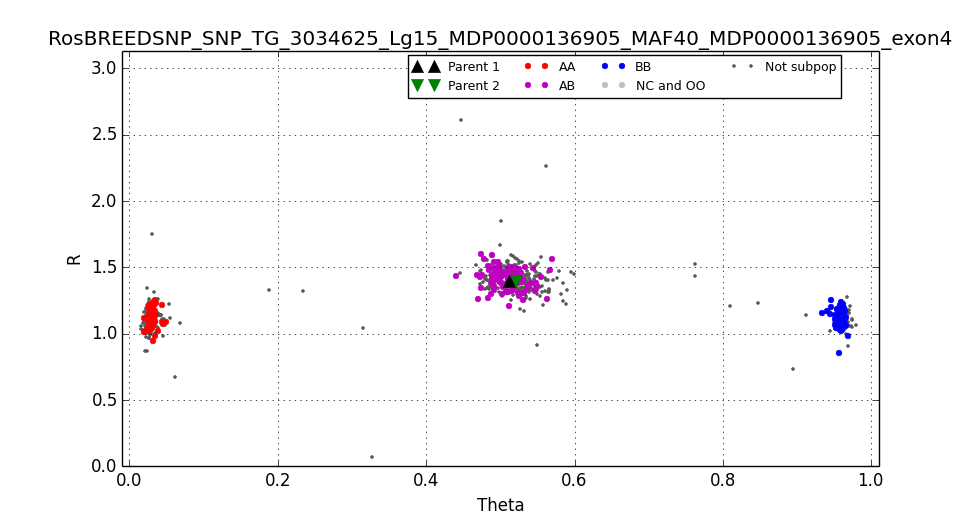
\includegraphics{_picture/robust.png}}
\caption{Plot of a Robust SNP.}\end{figure}

\item [NullAllele-Failed:] This class may appear when ``AB sub-clusters \& Null alleles''  is set
to ``Off''.  NullAllele-Failed are the SNPs in which the frequency of the
HomozygousNull genotypes (No Call with an intensity of the luminous signal, R,
lower than the threshold for null-alleles) is higher than the ``Unexpected genotype threshold per
SNP'' in ``CP (F1)'', BCx or F2 or higher than the ``Frequency rare allele'' in ``Germplasm''. 
When ``AB sub-clusters \& Null alleles'' is set to ``On'' the NullAllele-Failed are the SNPs in
which the frequency of HomozygousNull  exceeds the ``Unexpected genotype threshold per
SNP'', or for null-allele including segregation patterns that ASSIsT does not account for (see
last page of the manual), or when the segregation is too skewed (Chi-squared p-value lower than the
maximum allowed distortion) to fall in Null\_2\_Clusters or
Null\_4\_Clusters.
\begin{figure}[H]
\centering
\capstart

\scalebox{0.500000}{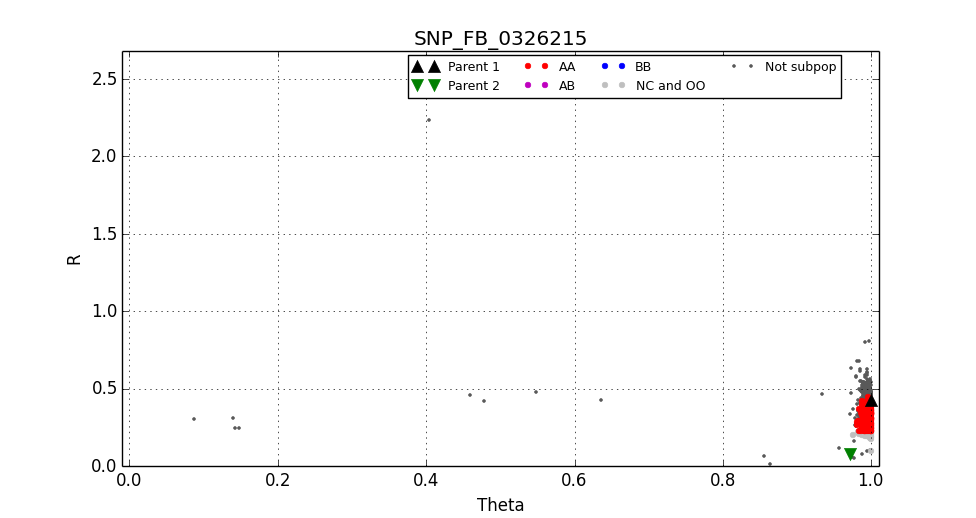
\includegraphics{_picture/NullAllele-Failed.png}}
\caption{Plot of a NullAllele-Failed SNP.}\end{figure}

\item [Null\_2\_Clusters:] SNPs fall in this category if the frequency of homozygous Null
genotypes is higher than the ``Unexpected genotype threshold per SNP'' and if the frequency of one
of the homozygous as well as heterozygous classes are lower than the ``Unexpected genotype
threshold per
SNP''. The presence of the null allele is coded with ``\emph{O}''. According to the genotypes of the
two parents it is possible to distinguish two different classes of markers: If parents are \emph{AO}
x \emph{OO}, half of the offspring will be \emph{AO} and half will be \emph{OO}. If both parents are
\emph{AO}, one quarter of the offspring will be \emph{AA}, half  will be \emph{AO} and one quarter 
will be \emph{OO}. \textbf{AA} and \textbf{AO} clusters are often partially or totally merged so
ASSIsT will score the marker according to the presence/absence of the \emph{A} allele in the
offspring.
This re-calling analysis results in two genotype configuration: \emph{A-}
(the second allele is not specified as it is not possible to determine whether the genotype is
\emph{AA} or \emph{AO}). This class can be present only in ``CP (F1)'' and ``BC'' populations
when ``AB sub-clusters \& Null alleles'' is set to ``On''.
Note that  ASSIST does not account for crosses of type \emph{AB} x \emph{OO} or \emph{AB} x
\emph{AO}.
\begin{figure}[H]
\centering
\capstart

\scalebox{0.500000}{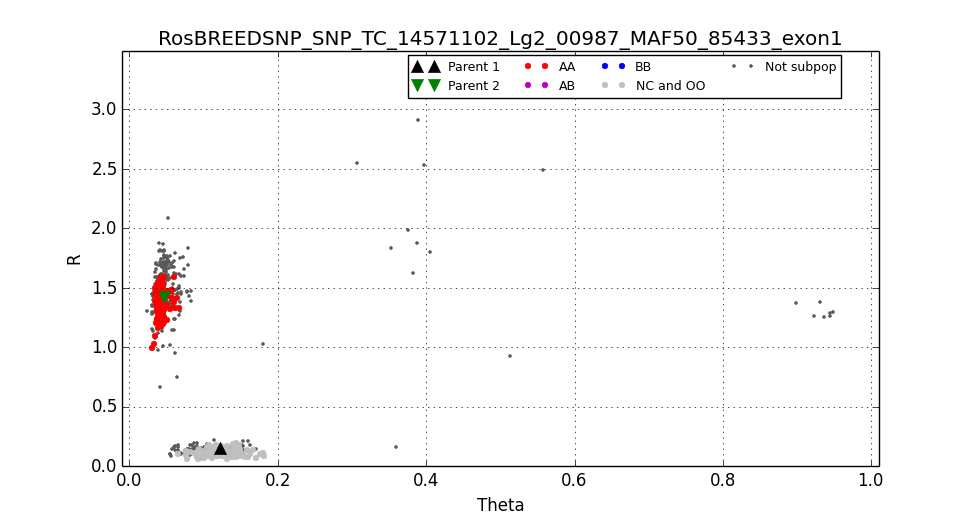
\includegraphics{_picture/Null-one-parent_2_Clusters.png}}
\caption{Plot of a Null-one-parent 2 Clusters SNP.}\end{figure}

\item [Null\_4\_Cluster:] SNPs fall in this category
when the frequencies of \emph{AA}, \emph{AB}, \emph{BB} and \emph{HomNull} 
(Both chromosomes with null allele) are higher than the ``Unexpected genotype threshold per
SNP'' and one of the parents is initially called AA and the other BB. Based on
the observed segregation pattern of the family (1 \emph{AA}: 1 \emph{AB}: 1 \emph{BB}: 1 \emph{OO}),
these parents are recoded
as \emph{AO} and \emph{BO}, and their progeny is  recoded as \emph{AO}, \emph{AB}, \emph{BO} and
\emph{OO}, respectively.
This class can be present only in a ``CP (F1)'' and ``BC'' population when
``AB sub-clusters \& Null alleles'' is set to ``On''.
\begin{figure}[H]
\centering
\capstart

\scalebox{0.500000}{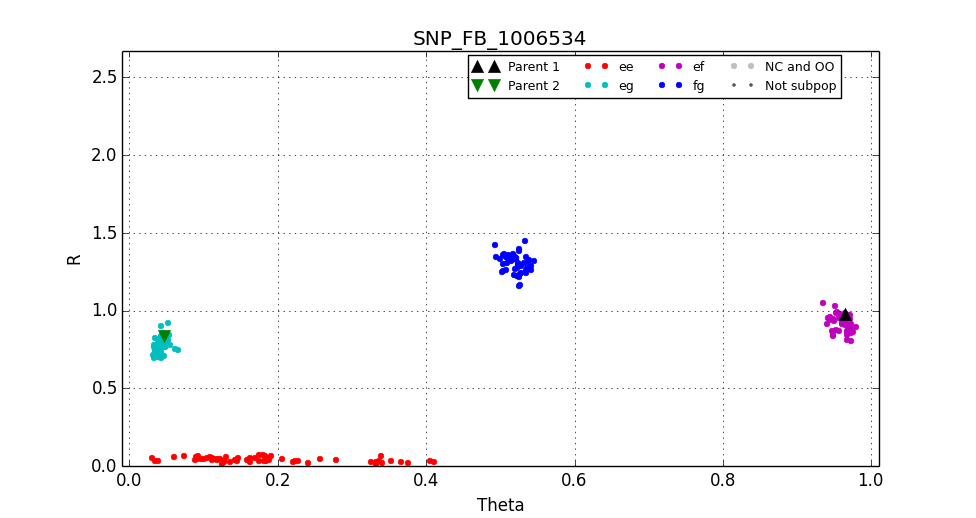
\includegraphics{_picture/Null-two-parents_4_Cluster.png}}
\caption{Plot of a Null-two-parents 4 Cluster SNP.}\end{figure}

\item [AB\_2\_sub-clusters:] The separation of the \emph{AB} cluster into two distinct sub-clusters
is tested when the ``AB sub-cluster \& NullAllele'' option is activated.
The presence of 2 sub-clusters within the \emph{AB}
genotypes is assessed by looking at the presence of one gap in the derivatives of the distances
between the
Theta of a contiguous data point. To exclude spurious separation at the lower or higher
bound of the \emph{AB} cluster, please be aware that the derivate is computed after a 10\% trim of
the extreme values of Theta.
The separation is accepted when less than three consecutive values are over 2 * 95th percentile
of the derivative distribution. This class can be present
only in the ``CP (F1)'' and ``BC'' populations.
\begin{figure}[H]
\centering
\capstart

\scalebox{0.500000}{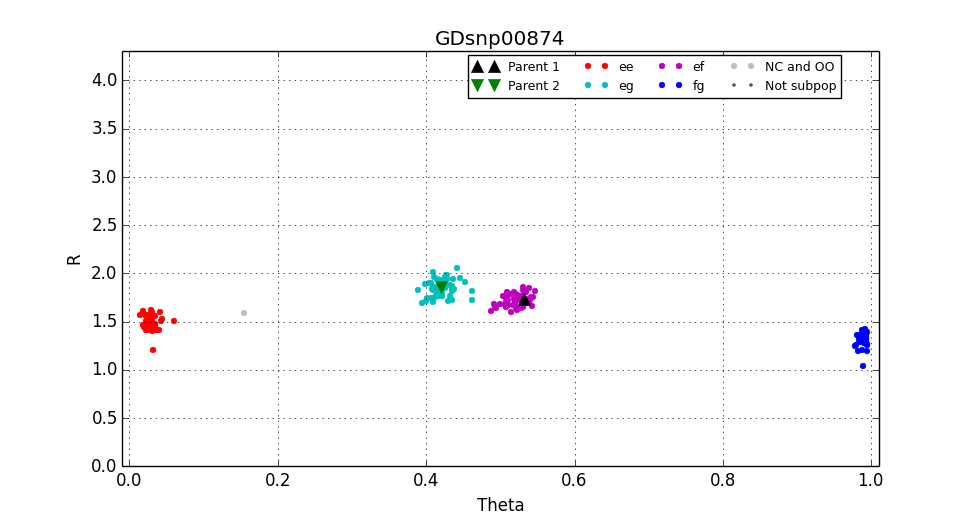
\includegraphics{_picture/AB_2_sub-clusters.png}}
\caption{Plot of a AB 2 sub-clusters SNP}\end{figure}

\item [OneHomozygRare\_HWE:] The SNPs are classified as ``OneHomozygRare\_HWE'' when the frequency
of one homozygote cluster is lower than the threshold for the ``Frequency rare allele''
but the proportions of the three genotype classes respect the Hardy-Weinberg equilibrium. This class
can be present only in the ``Germplasm'' population. In this case the ``Frequency rare allele'' is
actually used as genotype frequency and not as allelic frequency to warn the users about the
presence of clusters comprising few individuals. This situation in some cases can hide the presence
of an unspecific annealing that causes a shift of part of the homozygote cluster at higher or
lower Theta values in correspondence to the heterozygote cluster.

\item [OneHomozygRare\_NotHWE:] The SNPs are classified as ``OneHomozygRare\_\\NotHWE'' when the
frequency of one homozygote cluster is lower than the threshold for the ``Frequency rare
allele'' and the proportions of the three genotype classes does not follow the Hardy-Weinberg
equilibrium. This class can be present only
in the ``Germplasm'' population. In this case the ``Frequency rare allele'' is
actually used as genotype frequency and not as allelic frequency to warn the users about the
presence of clusters comprising few individuals. This situation in some cases can hide the presence
of an unspecific annealing that causes a shift of part of the homozygote cluster at higher or
lower Theta values in correspondence to the heterozygote cluster.

\begin{figure}[H]
\centering
\capstart

\scalebox{0.500000}{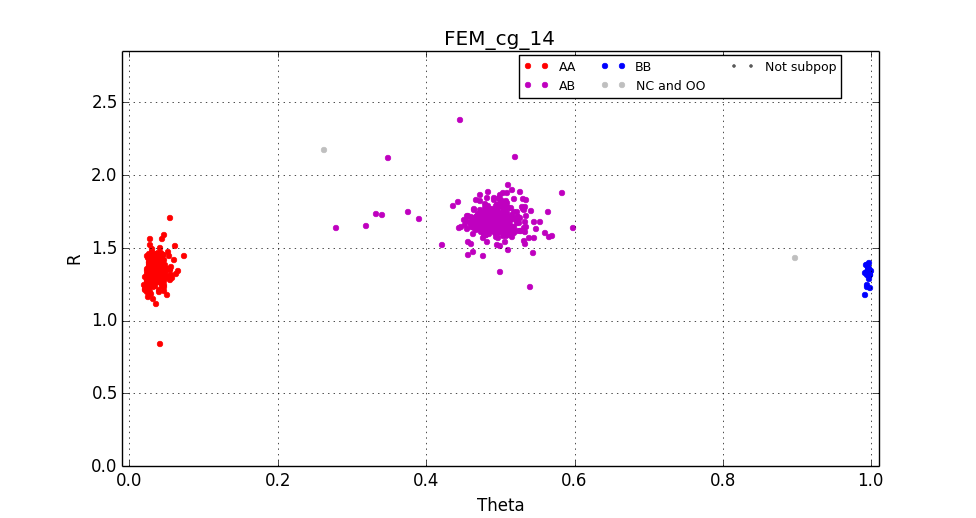
\includegraphics{_picture/oneHomoRare.png}}
\caption{Plot of a OneHomozygRare\_(Not)HWE SNP}\end{figure}

\item [Monomorphic:] The SNPs are classified as False-SNP when a single
Genotype  class is present  and its  frequency is higher than the rare allele
frequency threshold.
\begin{figure}[H]
\centering
\capstart

\scalebox{0.500000}{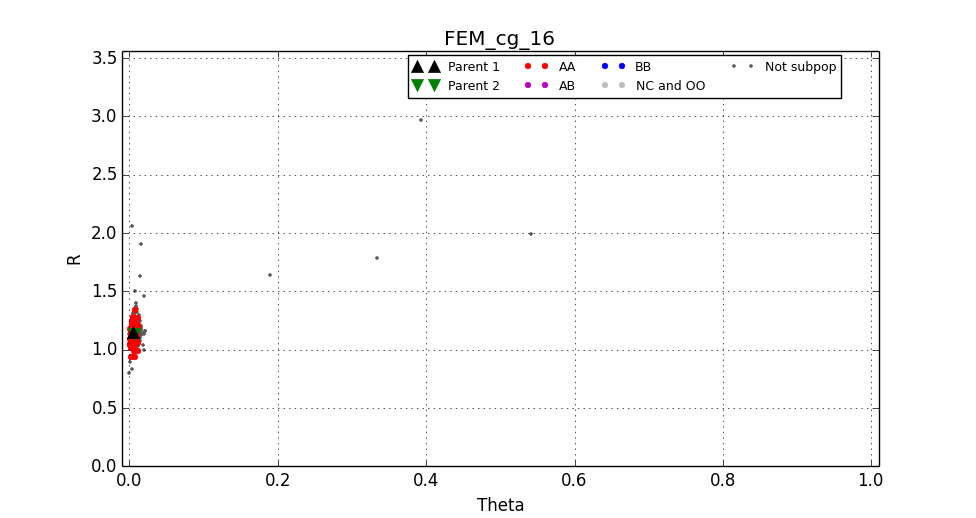
\includegraphics{_picture/Monomorphic(aaxaa).png}}
\caption{Plot of a Monomorphic SNP.}\end{figure}

\item [DistortedAndUnexpSegreg:] The segregation in the full-sib families shows a severe skewedness
(Chi-squared p-value higher than the value set in the parameters), or one of
the genotype classes is missing in a ``Germplasm'' population, or a genotype class occurs
which is not supported by the parental genotypes. This  could be due to for instance a AB x AO marker.
\begin{figure}[H]
\centering
\capstart

\scalebox{0.500000}{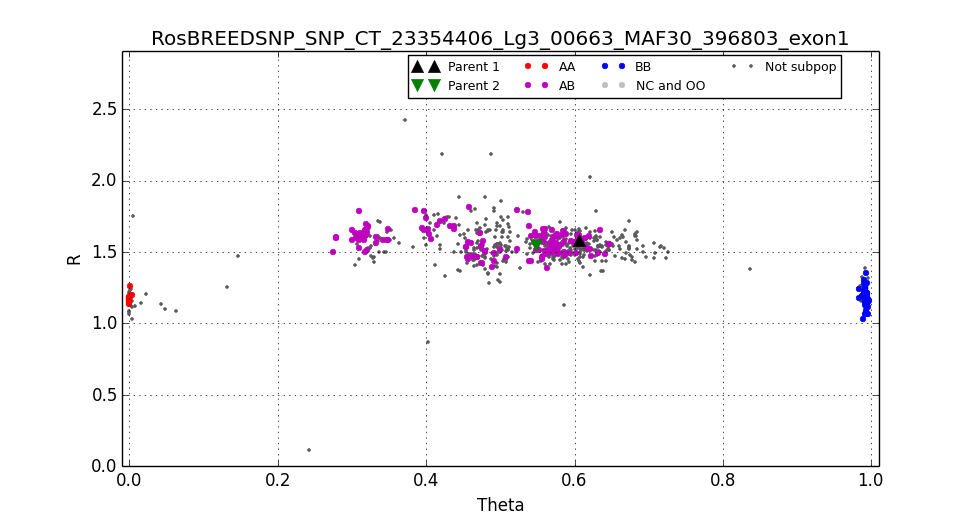
\includegraphics{_picture/Distorted.png}}
\caption{Plot of a Distorted SNP.}\end{figure}

\item [OneClassMissing:] In an ``F2'' population, SNPs fall into this class when one of the three
genotypes has a frequency lower than the rare allele frequency threshold.
\begin{figure}[H]
\centering
\capstart

\scalebox{0.500000}{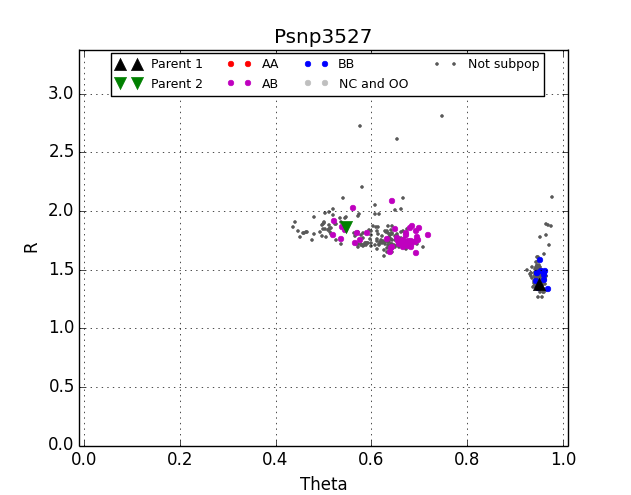
\includegraphics{_picture/oneClassMissing.png}}
\caption{Plot of a oneClassMissing SNP.}\end{figure}

\item [ShiftedHomo:] In a ``Germplasm'' population, SNPs are classified as ShiftedHomo when one of
the two homozygous classes is absent. This is normally due to an unspecific annealing that causes a
shift of the cluster at higher or lower Theta values, depending on the allele that is the concern
of the paralogy.
\begin{figure}[H]
\centering
\capstart

\scalebox{0.500000}{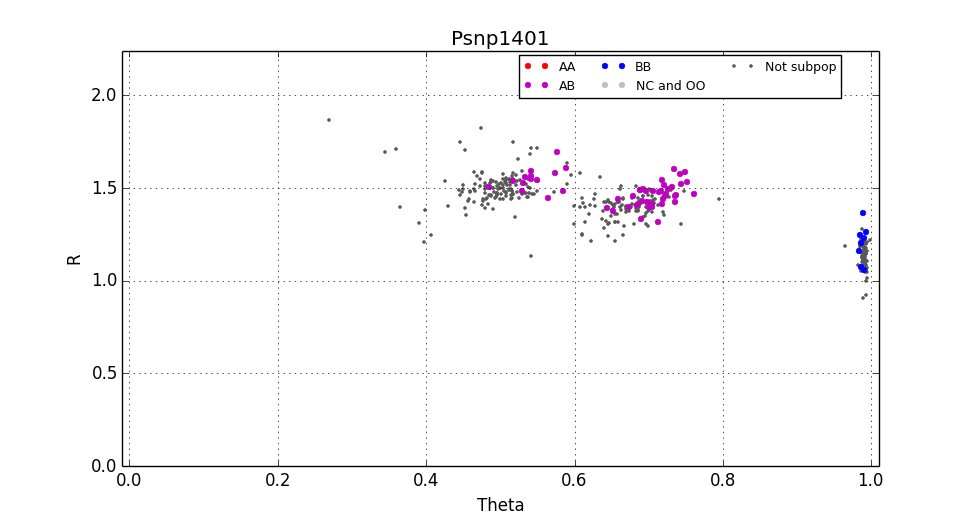
\includegraphics{_picture/shiftedHomo.png}}
\caption{Plot of a shiftedHomo SNP.}\end{figure}

\item [Failed:] All the SNPs that show a high rate of no-call, that have a mean signal intensity
\textless{}0.4
or that do not fall in any other class are classified as Failed.
\begin{figure}[H]
\centering
\capstart

\scalebox{0.500000}{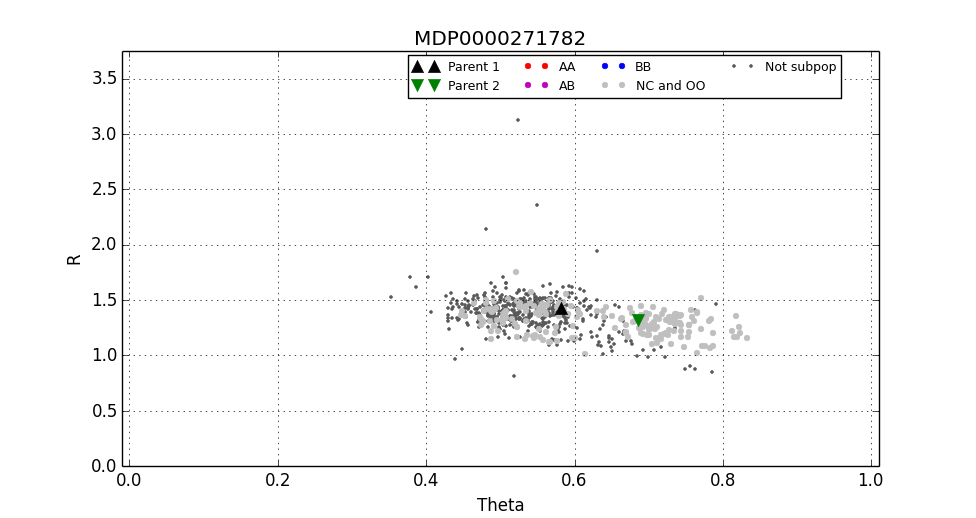
\includegraphics{_picture/Failed.png}}
\caption{Plot of a Failed SNP}\end{figure}

\end{description}


\section{Prospects for further development}
\label{index:prospects-for-further-development}


To our knowledge ASSIsT is the first software that identifies and calls null-alleles from SNP
markers. The parental SNP-genotype combinations considered are \emph{AO} x \emph{AO}, 
\emph{AO} x \emph{OO} and \emph{AO} x \emph{BO}.
The combinations \emph{AB} x \emph{AO} (\textbf{case (a)}) and \emph{AB} x \emph{OO}
(\textbf{case (b)}) 
do show equally good prospects based
on our results on SNP that were filtered and called  using Excel based procedures  developed
in-house.
These were not incorporated into ASSIsT due to time constraints. 

Currently, neither 
GenomeStudio\reg~ nor ASSIsT supports automated calling of SNP for which one of the clusters for
homozygous individuals (\emph{AA} or \emph{BB}) is in between x=0.4 and x=0.6, which is true for
part of the paralogous SNP.
Part of these SNP markers do show three well separated clusters (\textbf{case (c)}), and thus have
good
prospects for calling through alternative procedures.
Another useful extension could be the further classification of excluded markers. Currently, markers
with non-allowed genotypes and markers with segregation distortion are both assigned to the class
"Distorted and unexpected segregation".  

\begin{figure}[H]
      \captionsetup[subfigure]{}%labelformat=empty}
      %\caption{sweeppy}\label{fig:animals}
      %\centering
    	\begin{subfigure}[b]{0.5\textwidth}
          \caption{\emph{AO} x \emph{AB} \(\rightarrow\) \sfrac{1}{4} \emph{AO} + 
          \sfrac{1}{4} \emph{AA} + \sfrac{1}{4} \emph{AB} + \sfrac{1}{4} \emph{B0}}
           \scalebox{0.300000}{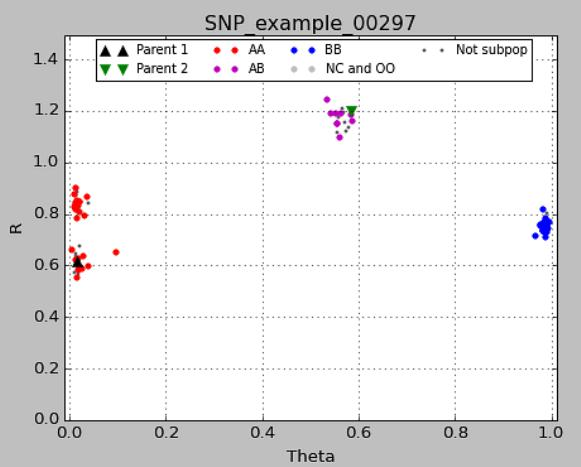
\includegraphics{_picture/furtherA}}
                \label{fig:gull}
        \end{subfigure}%
        ~
        \begin{subfigure}[b]{0.5\textwidth}
                \caption{\emph{OO} x \emph{AB} \(\rightarrow\) \sfrac{1}{2} \emph{AO} + 
          \sfrac{1}{2} \emph{BO}}
	\scalebox{0.300000}{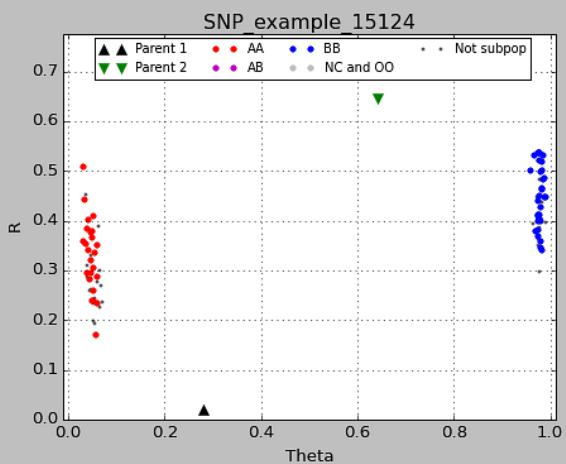
\includegraphics{_picture/furtherB}}
                \label{fig:tiger}
        \end{subfigure}
        \centering
        
        \bigskip
        
        \begin{subfigure}[b]{0.5\textwidth}
                \caption{\emph{AB} x \emph{AB} \(\rightarrow\) \sfrac{1}{4} \emph{AA} + 
          \sfrac{1}{2} \emph{AB} + \sfrac{1}{4} \emph{BB}}
                \scalebox{0.300000}{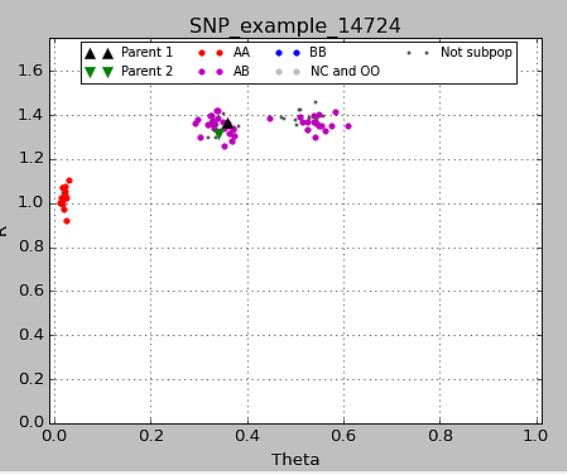
\includegraphics{_picture/furtherC}}
                \label{fig:mouse}
        \end{subfigure}
\label{fig:animals}
\end{figure}

\end{document}
